\begin{exercise}
In Example 4.1, suppose a new state $15$ is added to the gridworld just below state $13$, and its actions, $\mathit{left}, \mathit{up}$ $\mathit{right}$, and $\mathit{down}$, take the agent to states $12$, $13$, $14$, and $15$, respectively.
Assume that the transistions from the original states are unchnged.
What, then, ist $v_\pi(15)$ for the equiprobable random policy?
Now suppose the dynamics of state $13$ are also changed, such that action down from state $13$ takes the agent to the new state $15$.
What is $v_\pi(15)$ for the equiprobable random policy in this case?
\end{exercise}

\begin{solution}
If we use the bellman equations with parameter $\gamma = 1$ we get

\begin{align*}
  v_\pi(15)
  =
  \sum_{s^\prime \in \{12,13,14,15\}}\frac{1}{4}[-1 \cdot v_\pi(s^\prime)]
\end{align*}

We see that $v_\pi(15)$ is also in the sum, we do some algebraic manipulations to get

\begin{align*}
  v_\pi(15)
  =
  \frac{1}{3} \sum_{s^\prime \in \{12,13,14\}}[-1 \cdot v_\pi(s^\prime)] - \frac{1}{3}
\end{align*}

\begin{figure}[H]
  \centering
  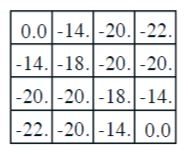
\includegraphics{Figure_4.1.jpg}
  \caption{Figure 4.1}
\end{figure}

If we take the values of the states $12,13$ and $14$ from Figure 4.1 in the Sutton and Barto textbook we get

\begin{align*}
  v_\pi(15)
  =
  -20
\end{align*}

If the dynamics of state $13$ are changed we get a whole new system of equations to solve.
\end{solution}
